\section{Applying it in Practice}

To show how the methods can be applied in practice, we discuss our implementation in this section.

To achieve full end-to-end AutoML for timeseries forecasting and anomaly detection that can be used by inexperienced users, we think there should be a custom built web application. A web application does not require any installation. Therefore, users do not have to setup a development environment or find a suitable cloud-based notebook solution or the like and then install a library, read the API documentation and start using it.

\newpage
The application should allow a user to specify the pipeline with as little configuration as possible. The main parts of our pipeline are the following:


\begin{itemize}
    \item \textbf{Sourcing:} In this step, the user must specify where the raw data can be retrieved from. 
    \item \textbf{Parsing:} It must be specified how the data should be read. This means telling something about the raw structure and for example which fields to read, which to ignore, and so forth.
    \item \textbf{Pre-Processing:} In the pre-processing step, the user must specify if they want to further process the raw data. This could for example be binning, time alignment, outlier cleaning, etc. but is optional.
    \item \textbf{Forecasting:} In this step, the model and its parameters are selected. This is where guided model selection comes into play and the user should be able to apply auto selection.
    \item \textbf{Anomaly Detection:} The optional step of anomaly detection uses the created forecasts and checks if new data, after the pre-processing step has run on it, matches the predictions, or lies outside the bounds. The user can accept the default sensitivity or specify a custom one.
    \item \textbf{Model Analyzer:} After the forecast was produced and new data comes in, the model analyzer can compute the error term this model had. This is a hidden step that the user does not see, except that there are metrics available per timeseries. We propose to have this step to be able to compare the performance of models over time. The analyzer can run on a schedule, intermittently or when requested by the system operators.
\end{itemize}

This pipeline should also allow to be be forked and joined between every step. Meaning, the user can define a sourcing and parsing step, and then based on the parsed data, they can define two pre-processing steps, each with different settings. This could for example be useful to create short-term forecasts with a higher resolution of e.g., hours, all the while creating long-term forecasts with a lower resolution of e.g., days. It might also be useful to join sources, if the original timeseries data is spread between different origins. Examples can be seen in figures \ref{fig:pipeline-join} and \ref{fig:pipeline-fork}.



\begin{figure*}
\centerline{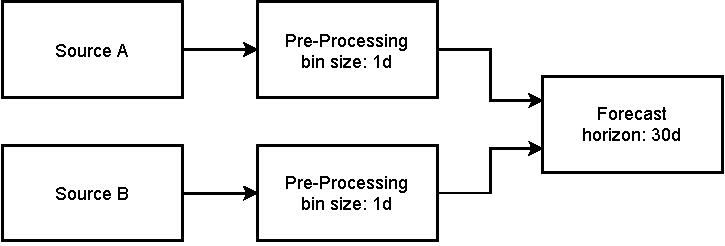
\includegraphics[scale=.7]{Figures/pipeline-join.pdf}}
\caption{Example of a pipeline that has two sources which are preprocessed independently, but then subsequently \emph{joined} to run in a single forecast step. It is the user's responsibility to ensure the sources are similar and make sense to be forecasted together.}
\label{fig:pipeline-join}
\end{figure*}


\begin{figure*}
\centerline{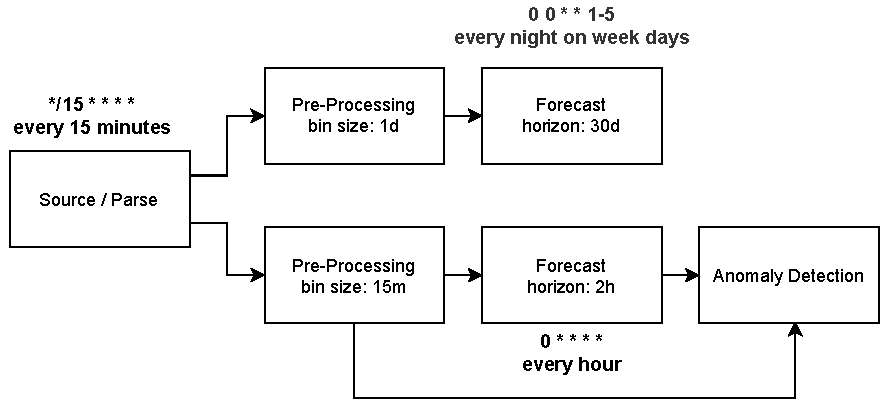
\includegraphics[scale=.7]{Figures/pipeline-fork.pdf}}
\caption{Example of a pipeline that has one source, after which the pipeline is \emph{forked}. This way users can create long-term forecasts and short-term forecasts for anomaly detection from the same source step. This means the raw data is only ingested once, which saves resources.}
\label{fig:pipeline-fork}
\end{figure*}

\subsection{Sourcing and Parsing}

The sourcing step needs to know how to retrieve raw data in the vague form of timeseries. 

This could for example be a URL that can be scraped and parsed. Or it could be a manually uploaded file. The tricky part is that the source could be in many forms. The file format could vary greatly, and even in the same file format, there are infinite possibilities to arrange the timeseries data. Thus, we must bring a lot of flexibility into the parsing step with a lot of configuration options. We also propose to split sourcing and parsing of the data. When the user is configuring a pipeline, they will need fast feedback. If they change the parsing configuration, the system should not need to download a large file again.

The aforementioned method of scraping is pull based whereas manual uploads are pushed based, although highly irregular. \emph{Pull} has the benefit of letting the system decide when to pull. This means there will never be back-pressure or processing lags in the system. However, it cannot guarantee the exact moments of data being scraped. Another drawback is that some external system needs to aggregate the data into timeseries in the first place. A push-based system, as it could be implemented with messaging techniques like Kafka, RabbitMQ and others, would benefit the producer of the data stream, as they do not need to put a metrics collection system in place. If necessary, a timeseries ingestion system such as InfluxDB, Prometheus, and so forth could be provided.

\subsection{Pre-Processing}

The pre-processing step is optional, and can transform the raw data, if desired or needed. Several pre-processing transformations make sense to apply, which cannot be figured out just by looking at the data.

Raw data can have various resolutions, and the user might be interested to collect data in higher resolutions. Thus, the pre-processing step can aggregate (also called binning) the data in bigger bins by summing or averaging the timeseries. Depending on the target bin size, it might also become relevant how those bins are aligned to time. E.g., a bin size of 15 minutes could be desired to be aligned to the full hour (0:00), the quarter hour (0:15) and so forth. We call this natural alignment which is nice for humans to consume. The analysis of the timeseries charts becomes more natural this way. The drawback when doing alignment is that the current time might not be containing all data of the most recent bin, thus this bin cannot be used yet. If we would include a partial last bin the charts will have a drop at the end, and the forecasts will most likely be heavily skewed. Consequently, if we do not include the last bin while it is of significant size yet, we cannot do near real time forecasting and anomaly detection anymore. Our recommendation would be to fork the pipeline and create two steps, one with natural alignment and one with current time alignment. The current time alignment data can be used to do near real time anomaly detection, while the naturally aligned data can be used for historical analysis.

Another pre-processing step is to fill missing data. Some models are not working well or at all when the timeseries contain missing data. Thus, by filling it in, we increase the number of models that will apply to our use case. Filling missing data in timeseries could be done with machine learning or statistical models. In fact that's how FEDOT \cite{fedot} started. As this data filling is not our main goal and only helps to increase model selection flexibility and pleases the human eye when they will later see a chart with a continuous, albeit straight line. Thus, we think back filling and forward filling are the only necessary options.

The source data could also be in absolute numbers, but the user is interested in differences per data point or vice versa. Thus, the pre-processing step should also be able to build new timeseries by building differences at various lags or to sum up differences to an absolute number (rolling sum). Some data might also be highly fluctuating, and the user would like to see smoothed data. So, moving averages of various lags should be configurable. It is important to apply these transformations before creating a forecast. One cannot assume that such a profound transformation does not affect the forecasters behavior. Our model selection will also likely suggest a different model.

Another important step besides smoothing is to explicitly remove outliers. There are several methods that can be used such as quantiles applied on sliding windows. More advanced methods, such as fitting a forecasting model are also possible, but they would be beside the point and not fast enough. We decided to use the Hampel filter \cite{HAMPEL}. It uses a sliding window. For each window of size $w$ we compute the median and the median absolute deviation (MAD). If point under observation has an $n_\sigma$-fold difference to the standard deviations, we treat it as an outlier. We can impute the point with the median to avoid missing data problems. This approach is simple, yet effective and fast. We preset the window size $w$ with 10 and $n_\sigma$ with 3. The user can adjust these parameters.

\subsection{Forecasting}

After data has been sourced, parsed and preprocessed we want to find a model for the data. The user needs to state the desired forecast horizon $fh$. The remaining features can be computed by each timeseries to figure out in which group it is. The user also needs to adjust the weights for accuracy, time/cost and explainability to create a ranking to their liking. The system will let the user choose the model of choice, if they wish to change the highest ranked model. Per timeseries, the model characteristics of accuracy, time and explainability are visible as a score $0-1$ and allow the user to base a decision on them. Scores are important for inexperienced users as they might not understand RMSSE or that different time series might lead to different CPU times required to fit the data. Once the model is chosen, the forecasting step invokes the forecaster to create a prediction for the desired horizon. The recommended model might change over time as more data is ingested. The user can enable auto selection. In this case the forecasting step first determines the group the timeseries lies in and chooses that model according to the users weights.

Some forecasters support computing prediction intervals. They are also called uncertainty bounds of the prediction. We want to store those bounds to be able to visualize them to a user. Some models do not support this feature and that's where we must use a benchmark method. We compute the standard deviation on the data that was incorporated into a forecast point. For Na\"ive this means that different values depending on the mode used (mean, last, drift). For other methods we compute the standard deviation of the window size.

Methods that support prediction intervals out of the box are Theta, ARIMA, Prophet, TBATS and BATS. If the user intends to append an anomaly detection step to this pipeline, it is recommended to use a method that properly supports intervals. Bounds produced by our benchmark method are rarely suitable to detect anomalies reliably. An example uncertainty interval is shown in figure \ref{fig:uncertainty}.


\begin{figure*}
\centerline{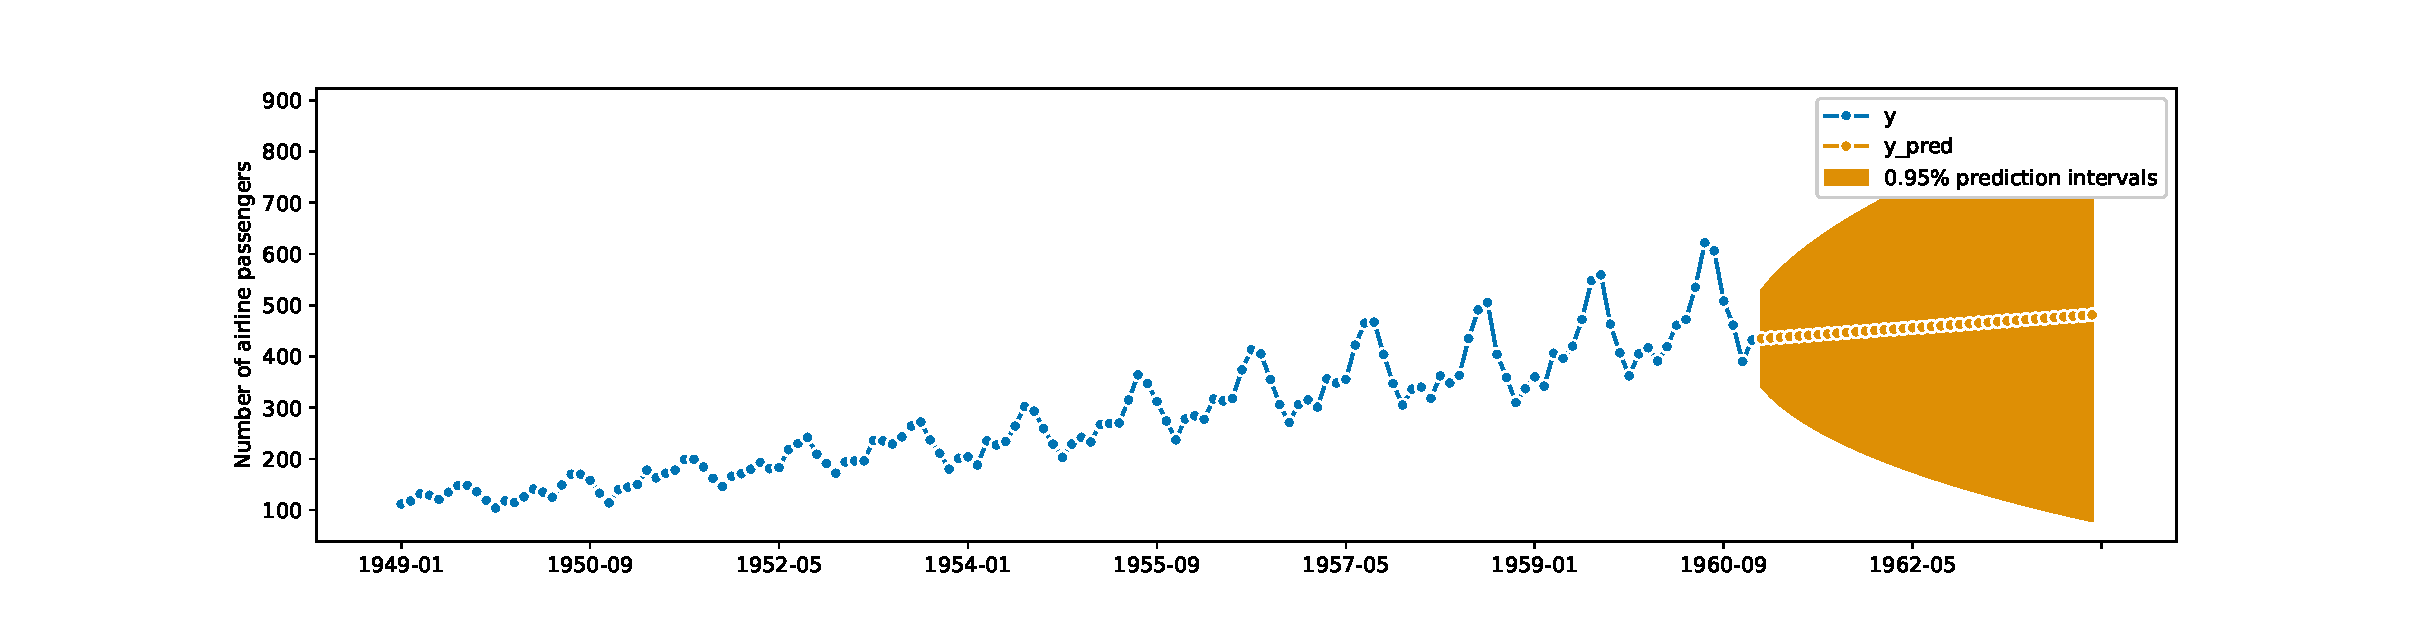
\includegraphics[scale=.5]{Figures/uncertainty.eps}}
\caption{This is an airline passenger example timeseries from sktime where we created a forecast and prediction intervals using a Theta forecaster. Uncertainty is an important factor when humans interpret a forecast. Often, forecasts can seem too correct, and humans tend to believe if they somehow find a reason to confirm the data is 100\% correct. We can also use prediction intervals to check if new data lies within the bounds or not to annotate it as an anomaly.}
\label{fig:uncertainty}
\end{figure*}

\subsection{Anomaly Detection}

The anomaly detection step uses new incoming data from the pre-processing step and compares it to the uncertainty intervals generated in the forecasting step. Users are additionally able to specify a sensitivity that can make the bounds produced by the model less strict and widen the area that is accepted to be no anomaly. A further configuration item is the duration an anomaly must occur. Traditionally anomalies are viewed as single points in a timeseries that are abnormal. But we also want to allow users to specify that something should only be regarded as an anomaly if there were a minimum of $n$ subsequent data points outside the bounds. Increasing this setting has the downside of removing the near-real-time anomaly detection aspect.

\subsection{Model Analyzer}

The model analyzer is collecting performance metrics of the forecasting method such as RMSSE by comparing training data and new data. This means that old forecasts need to be stored even though they are not used anymore, at least until the model analyzer has computed the necessary metrics.

Although we did not pursue this, by collecting these metrics, we could also run a different model on the same data without surfacing the results to the user. The model analyzer could then tell which model performed better. The system could be built to match up two competing models with every forecast until it finds the best forecaster given a timeseries in a bracket style evaluation.
